\scanpage{75}
dont le deuxième est donné par
\[(41)\qquad\boxed{\rho_1\unsure{\leftrightarrow}\sigma_\infty,\ \rho_\infty\longmapsto\rho^{-1},}\quad\rho_0=(\rho_\infty\rho_1)^{-1}\longmapsto\sigma_\infty\rho^{\unsure{\wedge}}=\varepsilon_0\]
et le premier par
\[(42)\qquad\boxed{\tau_{\deleted{\unsure{\infty}}}\longmapsto\tau_\infty},\quad\underset{\underset{\rho_0}{\Vert}}{\tau_{\deleted{\unsure{0}}}}\longmapsto\quad,\quad\boxed{\tau_\infty\longmapsto\tau_{\unsure{a}}}\quad,\]
\figure{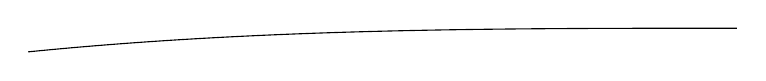
\begin{tikzpicture}\draw (0,0)..controls(3,.3)and(6,.3)..(9,.3);\end{tikzpicture}}
\figure{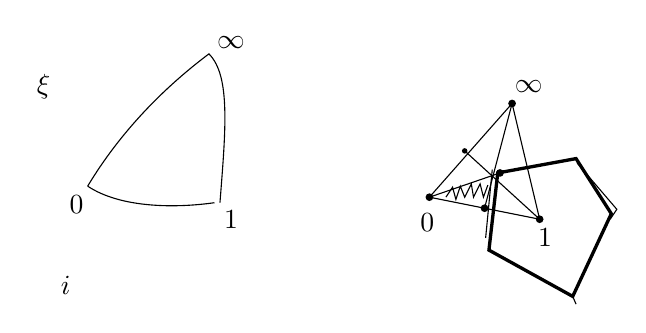
\begin{tikzpicture}[scale=1.4]
\node at(-.4,1.2){$\unsure{\xi}$};
\draw (0,.3)..controls(.3,.8)and(.7,1.2)..(1.1,1.5)..controls(1.3,1.3)and(1.25,.8)..(1.2,.15);
\draw (0,.3)..controls(.3,.1)and(.8,.1)..(1.15,.15);
\node at(-.1,.13){$0$};\node at(1.3,1.6){$\infty$};\node at(1.3,0){$1$};\node at(-.2,-.6){$\unsure{i}$};
\begin{scope}[xshift=3.1cm,yshift=-.2cm]
\draw (0,.4)--(.75,1.25)--(1,.2)--cycle;
\draw (0,.4)--(.64,.62);\draw (.75,1.25)--(.5,.3);\draw (1,.2)--(.32,.82);
\draw[very thick] (.62,.62)--(1.33,.75)--(1.65,.25)--(1.3,-.5)--(.54,-.08)--cycle;
\draw (.57,.65)--(.51,.03);\draw (1.3,-.5)--(1.33,-.57);\draw (1.34,.71)--(1.7,.29)--(1.64,.2);
\fill (0,.4)circle(.035);\fill (.75,1.25)circle(.035);\fill (1,.2)circle(.035);\fill (.64,.62)circle(.035);\fill (.5,.3)circle(.035);\fill (.32,.82)circle(.025);
\draw (.15,.4)--(.21,.49)--(.24,.38)--(.28,.5)--(.32,.4)--(.38,.52)--(.4,.4)--(.46,.52)--(.49,.4)--(.53,.51);
\node at(-.02,.17){$\unsure{0}$};\node at(.9,1.4){$\unsure{\infty}$};\node at(1.05,.03){$1$};
\end{scope}
\end{tikzpicture}}
\[\pi_{D_n},\quad\pi_{\widetilde G^+_4},\quad\pi_{\widetilde G_4},\quad\pi_{\widetilde G^+_5}\quad\unsure{-}\]
\[\pi_X\qquad\pi_X\longrightarrow X\ \text{une cat : \unsure{en excluant les sommets}}\]
\[\deleted{\pi_{\unsure{P_\infty}}}\qquad\pi_{\mathrm{icos}},\quad\pi_{\mathrm{dodéc}},\quad\pi_{\mathrm{tétr.}},\quad\pi_{\mathrm{cube}},\quad\pi_{\mathrm{oct.}},\quad\deleted{\pi_{\unsure{opicos}}}\]
\[\pi_{\unsure{\mathrm{paricos}}},\qquad\pi_P\longrightarrow\text{polygone combinatoire fini}\ldots\]
\mspage{74}
